\documentclass{rapport_gls}

\begin{document}

\begin{titlepage}
\begin{center}

% Titre
   \textsc{\Large ENSEEIHT : Génie du Logiciel et des Systèmes (GLS)}\\[6cm]
\textsc{\large Rapport retraçant les séances de TP}\\
\HRule \\
\huge{BE : Rapport de GLS\\}
\HRule \\[3cm]

\includegraphics[height=4cm]{../Images/gears.pdf}
\vfill

\LARGE{Matthieu Pizenberg}\\[1em]
\large{\today}

\end{center}
\end{titlepage}


\newpage

\tableofcontents

\newpage

\chapter{TP 2 : Méta-modélisation avec Eclipse/EMF}
\section{Comprendre les outils de métamodélisation d'Eclipse EMF}

Pour la prise en main des outils d'Eclipse on étudie le cas d'un modèle de procédé vu en td. Ce modèle suit un métamodèle simplePDL. Une première version de ce métamodèle est la suivante :

\begin{figure}[h]
   \centering
   \subfloat[modèle du sujet]{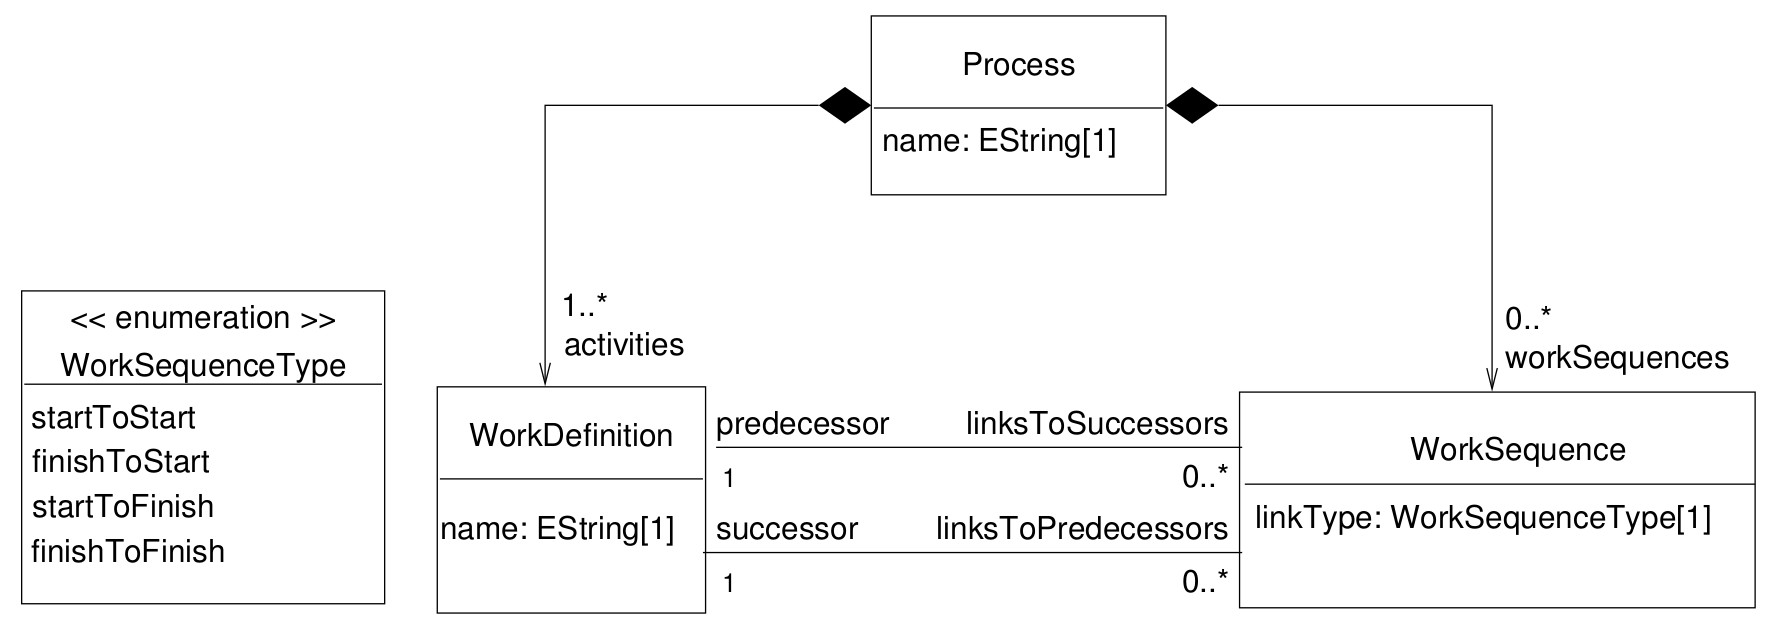
\includegraphics[width = 0.5\textwidth]{../Images/tp2/tp2_1-1.png}}
   \subfloat[diagramme du modèle ecore]{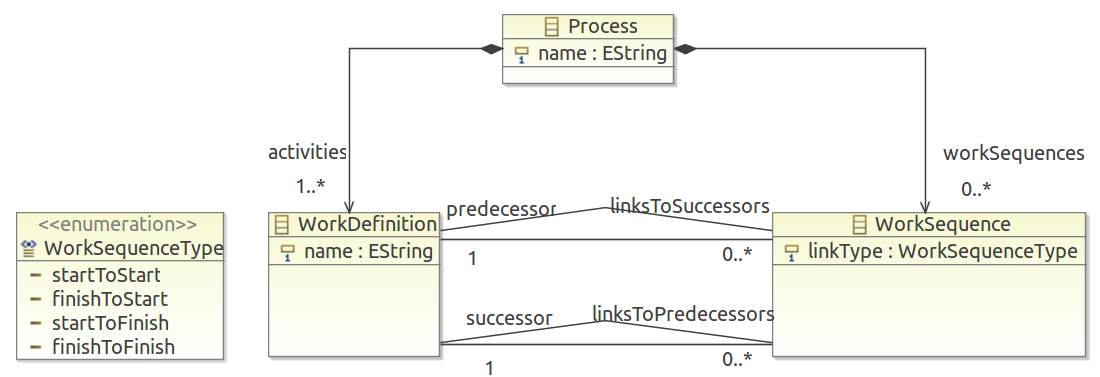
\includegraphics[width = 0.5\textwidth]{../Images/tp2/tp2_1-2.png}}
   \caption{Première version du métamodèle SimplePDL}
   \label{pdlv1}
\end{figure}

On utilise ensuite ce modèle avec l'éditeur réflexif (\textit{Create dynamic instance}) pour créer le modèle de procédé vu en td :

\begin{figure}[h]
   \centering
   \subfloat[Modèle de procédé]{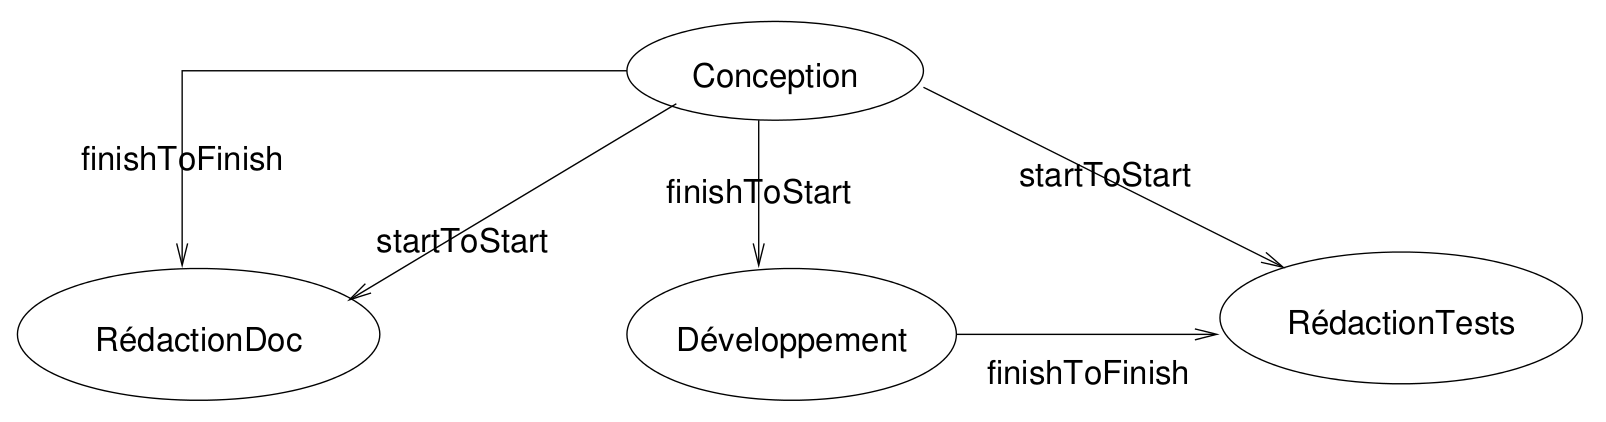
\includegraphics[width = 0.6\textwidth]{../Images/tp2/tp2_2-1.png}}
   \subfloat[Process.xmi]{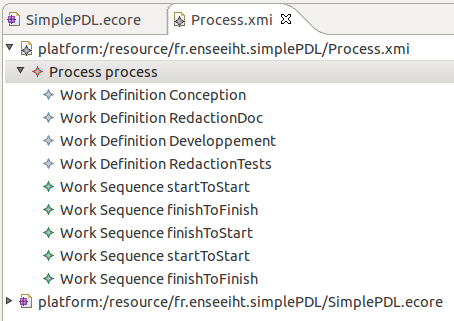
\includegraphics[width = 0.4\textwidth]{../Images/tp2/tp2_2-2.png}}
   \caption{Exemple de modèle de procédé}
   \label{process-1}
\end{figure}

\section{Compléter le métamodèle de SimplePDL}

On propose de compléter un peu le métamodèle de SimplePDL en ajoutant des \textit{ProcessElement} regrougant les \textit{WorkDefinition} et les \textit{WorkSequence} ainsi que d'ajouter la notion de \textit{Guidance} :

\begin{figure}[h]
   \centering
   \subfloat[Ancien modèle]{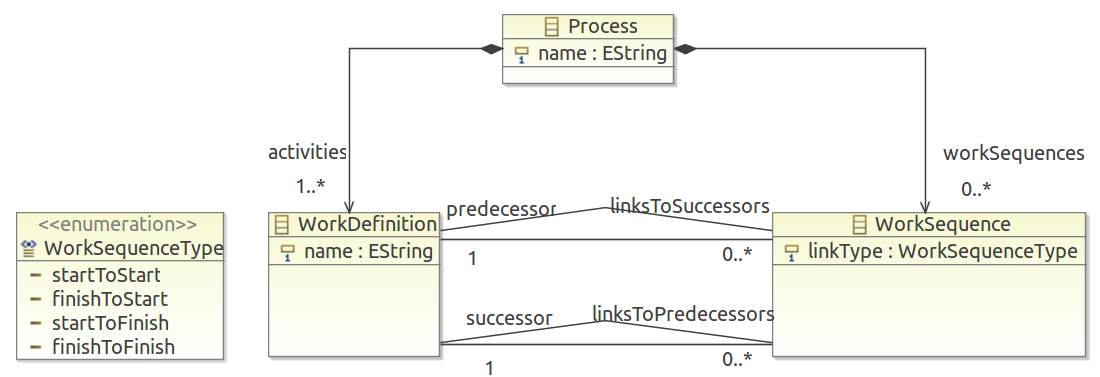
\includegraphics[width = 0.5\textwidth]{../Images/tp2/tp2_1-2.png}}
   \subfloat[Nouveau modèle]{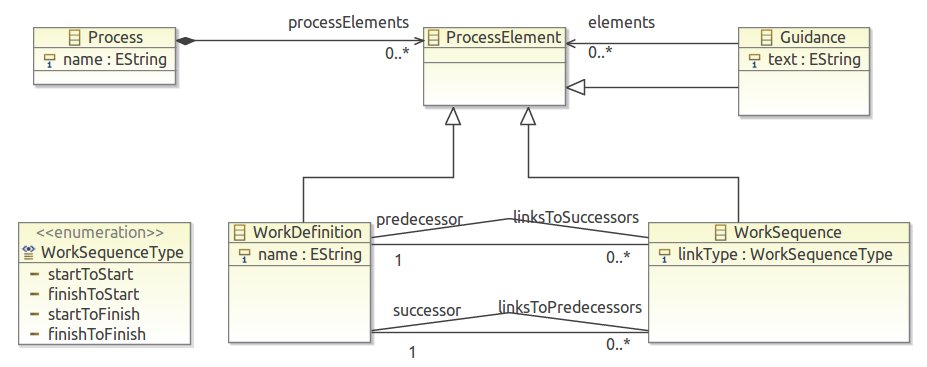
\includegraphics[width = 0.5\textwidth]{../Images/tp2/tp2_3-2.png}}
   \caption{Nouveau métamodèle de SimplePDL}
   \label{pdlv2}
\end{figure}

Le nouveau modèle permet d'ajouter plus de souplesse et de factoriser les propriétés communes aux éléments que l'on pourrait ajouter plus tard. Par contre cette factorisation regroupe l'ensemble des éléments sous le terme générique \textit{processElements} alors qu'on pouvait préciser avant \textit{activities} et \textit{WorkSequences}.

\section{Définir un métamodèle des réseaux de Petri}

On se propose maintenant de définir un métamodèle pour les réseaux de Petri.

\begin{figure}[h]
   \centering
   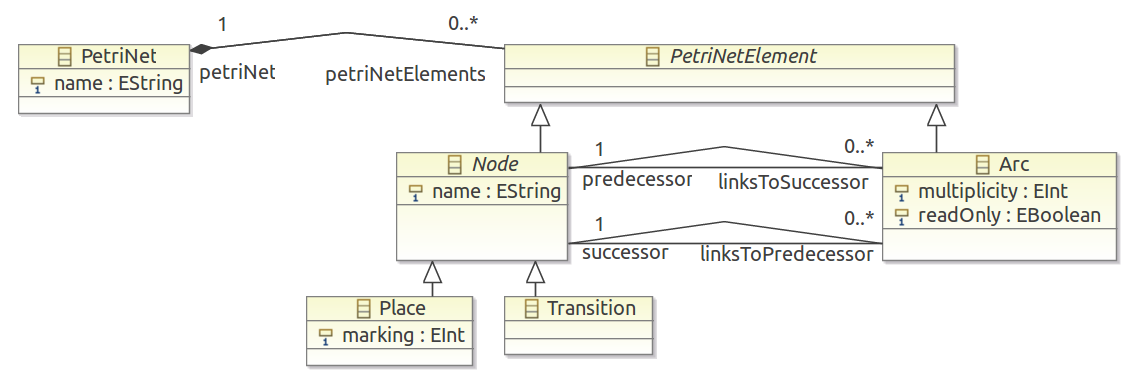
\includegraphics[width = 0.8\textwidth]{../Images/tp2/tp2_4.png}
   \caption{proposition de modèle pour les réseaux de Petri}
   \label{petriModel}
\end{figure}

Ce métamodèle est plus général que celui des réseaux de Petri. Un modèle suivant ce métamodèle peut par exemple avoir un arc reliant 2 places ou 2 transitions ce qui ne devrait pas être possible pour un réseau de Petri. On pourra cependant donner des restrictions et des règles avec le langage OCL pour ne décrire que des réseaux de Petri.

\chapter{TP 3 : Sémantique statique d'un DSML avec OCL}
\section{Compléter un métamodèle par des contraintes statiques}

Le fichier OCLinEcore est la description du métamodèle dans la syntaxe OCL. On remarque les correspondances suivantes :
\begin{itemize}
   \item Les classes Process, WorkDefinition, WorkSequence et Guidance sont déclarées en tant que "class"
   \item ProcessElement est une "abstract class"
   \item L'énumération WorkSequenceType est déclarée avec le mot clé "enum", les éléments sont énumérés avec "literal", chacun étant mis en correspondance avec un entier
   \item L'héritage entre les classes est déclarée avec le mot-clé "extends"
   \item On déclare les attributs avec le mot clé "attribute" et les relations avec "property"
   \item la relation containment est exprimée en ajoutant "composes" à une propriété
\end{itemize}

\vspace{1em}
On ajoute ensuite des contraintes OCL avec le mot clé "invariant". Les contraintes ajoutées sont les suivantes :
\begin{enumerate}
   \item "sameWDName" : deux activités différentes d'un même processus ne peuvent avoir le même nom.
   \item "reflexivity" : une dépendance ne peut pas être réflexive.
   \item "voidName" : le nom d'une activité doit être composé d'au moins un caractère.
\end{enumerate}

\vspace{1em}
Leur codes correspondants sont les suivants :
\begin{lstlisting}[caption="sameWDName" in Process class]
invariant sameWDName : (self.processElements)
   ->select(p|p.oclIsTypeOf(WorkDefinition))
   ->forAll(j,k | j<>k implies j.name <> k.name);
\end{lstlisting}

\begin{lstlisting}[caption="reflexivity" in WorkSequence class]
invariant reflexivity : self.predecessor <> self.successor;
\end{lstlisting}

\begin{lstlisting}[caption="voidName" in WorkDefinition class]
invariant voidName : name <> '';
\end{lstlisting}

\section{Application aux réseaux de Petri}

Comme prévu au tp précédent on ajoute les contraintes OCL suivantes à notre modèle de réseaux de Petri :

Dans la classe PetriNet :
\begin{itemize}
   \item "voidPetriName" : le nom d'un réseau de Petri doit avoir au moins 1 caractère
   \item "sameNodeName" : les places et les transitions doivent avoir des noms différents
\end{itemize}

Dans la classe Node :
\begin{itemize}
   \item "voidNodeName" : les noms des places et des transitions doivent avoir au moins 1 caractère
\end{itemize}

Dans la classe Arc :
\begin{itemize}
   \item "previousNodeNotInSamePetriNet" : le noeud précédent (place ou transition) est dans le même réseau de Petri
   \item "nextNodeNotInSamePetriNet" : le noeud suivant (place ou transition) est dans le même réseau de Petri
   \item "placeToTransition" : un arc venant d'une place arrive sur une transition
   \item "transitionToPlace" : un arc venant d'une transition arrive sur une place
\end{itemize}

\vspace{2em}
Le fichier PetriNet.ecore est le suivant :
\begin{lstlisting}[caption=PetriNet.ecore]
module _'PetriNet.ecore'
import ecore : 'http://www.eclipse.org/emf/2002/Ecore#/';

package petrinet : petrinet = 'http://petrinet/1.0'
{
   class PetriNet
   {
      invariant voidPetriName: name <> '';
      invariant sameNodeName:
      self.petriNetElements->select(p : PetriNetElement | p.oclIsKindOf(Node))->forAll(j : Node, k : Node | j <> k implies j.name <> k.name);
      attribute name : String[1] { ordered };
      property petriNetElements#petriNet : PetriNetElement[*] { ordered composes };
   }
   abstract class PetriNetElement
   {
      property petriNet#petriNetElements : PetriNet[1] { ordered };
   }
   abstract class Node extends PetriNetElement
   {
      invariant voidNodeName: name <> '';
      property linksToSuccessor#predecessor : Arc[*] { ordered };
      property linksToPredecessor#successor : Arc[*] { ordered };
      attribute name : String[1] { ordered };
   }
   class Arc extends PetriNetElement
   {
      invariant transitionToPlace: self.predecessor.oclIsTypeOf(Transition) implies self.successor.oclIsTypeOf(Place);
      invariant previousNodeNotInSamePetriNet: self.petriNet = self.predecessor.petriNet;
      invariant nextNodeNotInSamePetriNet: self.petriNet = self.successor.petriNet;
      invariant placeToTransition: self.predecessor.oclIsTypeOf(Place) implies self.successor.oclIsTypeOf(Transition);
      property predecessor#linksToSuccessor : Node[1] { ordered };
      property successor#linksToPredecessor : Node[1] { ordered };
      attribute multiplicity : ecore::EInt[1] { ordered };
      attribute readOnly : Boolean[1] { ordered };
   }
   class Place extends Node
   {
      attribute marking : ecore::EInt[1] { ordered };
   }
   class Transition extends Node;
}
\end{lstlisting}

\chapter{TP 4 : Transformation de modèle à texte}
%L'objectif de ce TP est de pouvoir transformer un modèle en texte à l'aide de l'outil Acceleo.

\section{Transformation de modèle à texte avec Acceleo}

Dans un premier temps on s'intéresse aux transformations à partir de modèle simplePDL.
Ces modèles sont exportés dans des fichiers textes respectant la syntaxe PDL1 et la syntaxe DOT.\\

Voilà par exemple le template pour la syntaxe PDL1 :\\

\lstset{language={}}
\begin{lstlisting}[caption=toPDL1.mtl]
[comment encoding = UTF-8 /]
[module toPDL1('http://simplepdl')]

[comment Generation de la syntaxe PDL1 à partir d'un modèle de processus /]

[template public toPDL(proc : Process)]
[comment @main/]
[file (proc.name.concat('.pdl1'), false, 'UTF-8')]
process [proc.name/]{
[for (wd : WorkDefinition | proc.processElements->getWDs())]
   wd [wd.name/]
[/for]
[for (ws : WorkSequence | proc.processElements->getWSs())]
   ws [ws.predecessor.name/] [ws.getWSType()/] [ws.successor.name/]
[/for]
}
[/file]
[/template]

[query public getWDs(elements : OrderedSet(ProcessElement)) : OrderedSet(WorkDefinition) = 
   elements->select( e | e.oclIsTypeOf(WorkDefinition) )
      ->collect( e | e.oclAsType(WorkDefinition) )
      ->asOrderedSet()
/]

[query public getWSs(elements : OrderedSet(ProcessElement)) : OrderedSet(WorkSequence) = 
   elements->select( e | e.oclIsTypeOf(WorkSequence) )
      ->collect( e | e.oclAsType(WorkSequence) )
      ->asOrderedSet()
/]

[template public getWSType(ws : WorkSequence)]
[if (ws.linkType = WorkSequenceType::startToStart)]
s2s[elseif (ws.linkType = WorkSequenceType::startToFinish)]
s2f[elseif (ws.linkType = WorkSequenceType::finishToStart)]
f2s[elseif (ws.linkType = WorkSequenceType::finishToFinish)]
f2f[/if]
[/template]

\end{lstlisting}

Les principales structures que l'on remarque sont les "template" qui permettent de mettre en page dynamiquement des bouts de code avec les objets transmis en paramètre et les "query" qui permettent de récupérer des ensembles sur lesquels on pourra itérer.\\

En s'inspirant de ce modèle, j'ai fait un template pour la transformation vers fichier ".dot".

\begin{lstlisting}[caption=toDot.mtl]
[comment encoding = UTF-8 /]
[module toDot('http://simplepdl')]

[comment Generation de la syntaxe dot à partir d'un modèle de processus /]

[template public toDot(proc : Process)]
[comment @main/]
[file (proc.name.concat('.dot'), false, 'UTF-8')]
digraph [proc.name/]{
[for (ws : WorkSequence | proc.processElements->getWSs())]
	[ws.predecessor.name/]->[ws.successor.name/]
[/for]
}
[/file]
[/template]

[query public getWSs(elements : OrderedSet(ProcessElement)) : OrderedSet(WorkSequence) = 
	elements->select( e | e.oclIsTypeOf(WorkSequence) )
		->collect( e | e.oclAsType(WorkSequence) )
		->asOrderedSet()
/]
\end{lstlisting}

Avec ce template on peut transformer le modèle de processus suivant en format texte :

\begin{center}
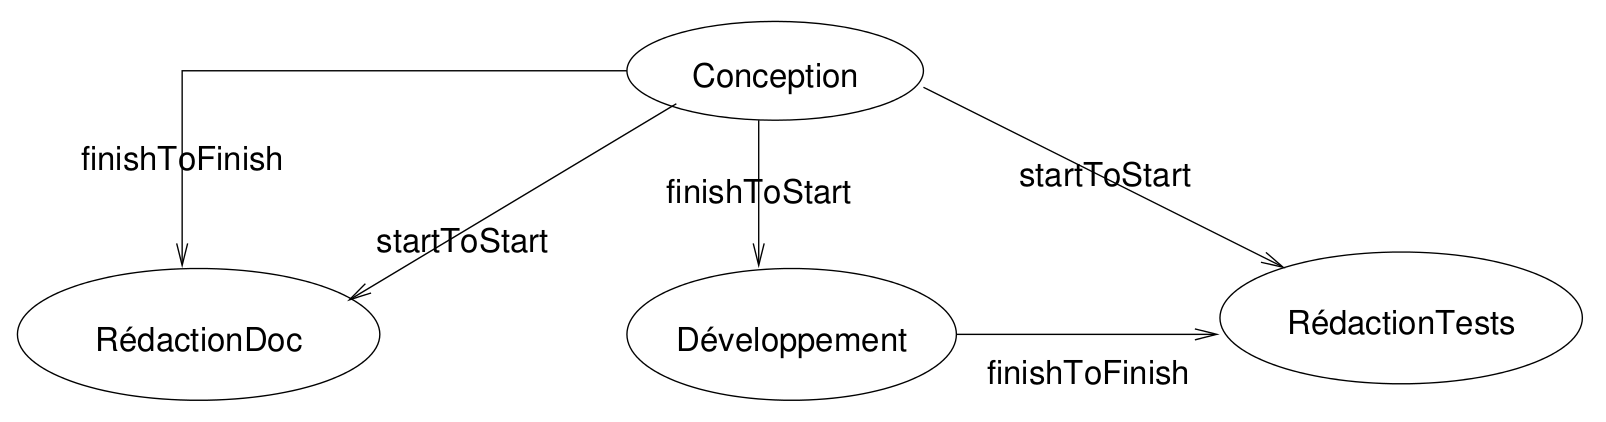
\includegraphics[width = 0.5\textwidth]{../Images/tp2/tp2_2-1.png}
\end{center}

et on obtient :

\begin{lstlisting}[caption=process.dot]
digraph process{
	Conception->RedactionDoc
	Conception->RedactionDoc
	Conception->Developpement
	Conception->RedactionTests
	Developpement->RedactionTests
}
\end{lstlisting}

\section{Application aux réseaux de Petri}

On transforme maintenant des modèles de réseau de pétri en texte. On fera un template pour fichier".net" et un template pour fichier ".dot". Le modèle de réseau de pétri nous servant d'example sera le même que celui du sujet, à savoir :

\begin{center}
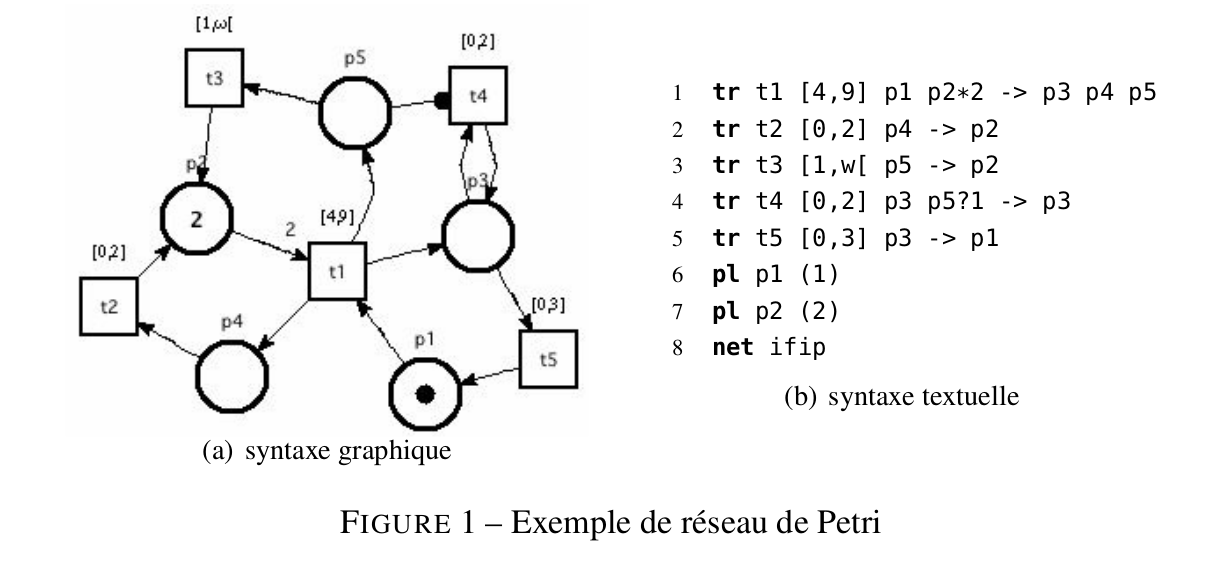
\includegraphics[width = 0.9\textwidth]{../Images/tp4/tp4_1.png}
\end{center}

On obtient les fichiers texte suivants :

\begin{lstlisting}[caption=example.net]
tr t1 p1 p2*2 -> p3 p4 p5
tr t2 p4 -> p2
tr t3 p5 -> p2
tr t4 p3 p5?1 -> p3
tr t5 p3 -> p1
pl p1 (1)
pl p2 (2)
net example
\end{lstlisting}

\begin{lstlisting}[caption=example.dot]
digraph example {
	t1 [shape=box];
	t2 [shape=box];
	t3 [shape=box];
	t4 [shape=box];
	t5 [shape=box];

	p1 [label="1"]
	p2 [label="2"]
	p3 [label=" "]
	p4 [label=" "]
	p5 [label=" "]

	p1 -> t1;
	p2 -> t1 [label="2"] ;
	p3 -> t4;
	p3 -> t5;
	p4 -> t2;
	p5 -> t3;
	p5 -> t4;
	t1 -> p3;
	t1 -> p4;
	t1 -> p5;
	t2 -> p2;
	t3 -> p2;
	t4 -> p3;
	t5 -> p1;
}
\end{lstlisting}

Le fichier example.dot une fois affiché donne ceci :

\begin{center}
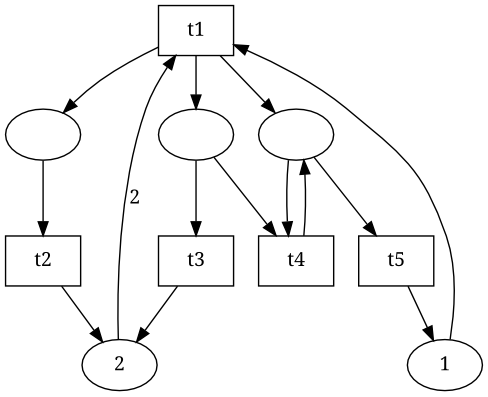
\includegraphics[width = 0.5\textwidth]{../Images/tp4/example.png}
\end{center}

On remarque que certaines améliorations sont possibles. On pourrait par example changer la couleur d'un read-arc et ajouter le nom d'une place en plus de son marquage dans les places.

Les codes des templates sont les suivants :

\begin{lstlisting}[caption=toNet.mtl]
[comment encoding = UTF-8 /]
[module toNet('http://petrinet/1.0')]

[comment Generation de la syntaxe .net à partir d'un modèle de réseau de pétri /]

[template public toNet(petriNet : PetriNet)]
[comment @main/]
[file (petriNet.name.concat('.net'), false, 'UTF-8')]
[for (tr : Transition | petriNet.petriNetElements->getTransitions())]
tr [tr.name/][tr.getTransitionsPredecessors()/] ->[tr.getTransitionsSuccessors()/]
[/for]
[for (pl : Place | petriNet.petriNetElements->getPlaces())]
[if (pl.marking > 0)]pl [pl.name/] ([pl.marking/])[/if]
[/for]
net [petriNet.name/]
[/file]
[/template]

[query public getTransitions(elements : OrderedSet(PetriNetElement)) : OrderedSet(Transition) = 
	elements->select( e | e.oclIsTypeOf(Transition) )
		->collect( e | e.oclAsType(Transition) )
		->asOrderedSet()
/]

[query public getPlaces(elements : OrderedSet(PetriNetElement)) : OrderedSet(Place) = 
	elements->select( e | e.oclIsTypeOf(Place) )
		->collect( e | e.oclAsType(Place) )
		->select( e | e.marking > 0 )
		->asOrderedSet()
/]

[template public getTransitionsPredecessors(tr : Transition)]
[for (arc : Arc | tr.linksToPredecessor)] [arc.getPredecessorPlace()/][/for]
[/template]

[template public getTransitionsSuccessors(tr : Transition)]
[for (arc : Arc | tr.linksToSuccessor)] [arc.getSuccessorPlace()/][/for]
[/template]

[template public getPredecessorPlace(arc : Arc)]
[arc.predecessor.name/][if (arc.readOnly)]?[arc.multiplicity/][elseif (arc.multiplicity > 1)]*[arc.multiplicity/][/if]
[/template]

[template public getSuccessorPlace(arc : Arc)]
[arc.successor.name/][if (arc.multiplicity > 1)]*[arc.multiplicity/][/if]
[/template]
\end{lstlisting}

\begin{lstlisting}[caption=toDot.mtl]
[comment encoding = UTF-8 /]
[module toDot('http://petrinet/1.0')/]

[comment Generation de la syntaxe .dot à partir d'un modèle de réseau de pétri /]

[template public toDot(petriNet : PetriNet)]
[comment @main/]
[file (petriNet.name.concat('.dot'), false, 'UTF-8')]
digraph [petriNet.name/] {
	[for (tr : Transition | petriNet.petriNetElements->getTransitions())]
	[tr.name/] ['box'.getShape()/];
	[/for]

	[for (pl : Place | petriNet.petriNetElements->getPlaces())]
	[pl.name/] [if (pl.marking > 0)][pl.marking.toString().getLabel()/][else][' '.getLabel()/][/if]
	[/for]

	[for (arc : Arc | petriNet.petriNetElements->getArcs())]
	[arc.predecessor.name/] -> [arc.successor.name/][if (arc.multiplicity > 1)] [arc.multiplicity.toString().getLabel()/] [/if];
	[/for]
}
[/file]
[/template]

[query public getTransitions(elements : OrderedSet(PetriNetElement)) : OrderedSet(Transition) = 
	elements->select( e | e.oclIsTypeOf(Transition) )
		->collect( e | e.oclAsType(Transition) )
		->asOrderedSet()
/]

[query public getPlaces(elements : OrderedSet(PetriNetElement)) : OrderedSet(Place) = 
	elements->select( e | e.oclIsTypeOf(Place) )
		->collect( e | e.oclAsType(Place) )
		->asOrderedSet()
/]

[query public getArcs(elements : OrderedSet(PetriNetElement)) : OrderedSet(Arc) = 
	elements->select( e | e.oclIsTypeOf(Arc) )
		->collect( e | e.oclAsType(Arc) )
		->asOrderedSet()
/]

[template public getLabel(s : String)]
['['/]label="[s/]"[']'/]
[/template]

[template public getShape(s : String)]
['['/]shape=[s/][']'/]
[/template]
\end{lstlisting}


\chapter{TP 5 : Eclipse Modeling Framework (EMF)}
%\input{tp5.tex}
\chapter{TP 6 : Définition de syntaxes concrètes textuelles}
%\input{tp6.tex}
\chapter{TP 7 : Définition de syntaxes concrètes graphiques}
%\input{tp7.tex}
\chapter{TP 8 : Transformation de modèle à modèle}
%\input{tp8.tex}

\end{document}
